\documentclass{article}
\usepackage{amsmath}
\usepackage{multicol}
\usepackage{geometry}
\usepackage{graphicx}
\usepackage{mathtools}
\usepackage{fancyhdr}
\graphicspath{ {./images/} }

\setlength{\columnsep}{1cm}
\setlength{\columnseprule}{1pt}

\expandafter\def\expandafter\normalsize\expandafter{%
    \normalsize%
    \setlength\abovedisplayskip{0pt}%
    \setlength\belowdisplayskip{9pt}%
    \setlength\abovedisplayshortskip{0pt}%
    \setlength\belowdisplayshortskip{10pt}%
}


\title{\vspace{-100pt} \Huge Formulario Física. Selectividad(Andalucía)}
\author{}
\date{}

\geometry{
  left=1cm,
  right=1cm,
  bottom=1.5cm
}


\fancyhf{}
\fancyhead[C]{\Large Formulario Física - Selectividad(Andalucía)}
\fancyfoot[R]{Javier Torralbo Cortés (javiertorralbocortes@gmail.com)}
\renewcommand\headrulewidth{1pt}
\renewcommand\footrulewidth{1pt}
\pagestyle{fancy}


\begin{document}
\centering

\begin{multicols}{2}[] 

\section{Campo gravitatorio}

\begin{center}
  \begin{tabular}{|c|c|}
      \hline
      $\vec{F}=-G\frac{Mm}{R^2}\cdot\vec{u}_R(N)$ & $\vec{Ep}=-G\frac{Mm}{R}(J)=mV$ \\
      \hline
      $\vec{g}=-G\frac{M}{R^2}\cdot\vec{u}_R(\frac{N}{kg})$ & $\vec{V}=-G\frac{M}{R}(\frac{J}{kg})$ \\
      \hline
      $W=-\Delta Ep$ & $W=-m\Delta V$ \\
      \hline
   \end{tabular}
\end{center}


Fuerza centrífuga:
\[F_c=\frac{m\cdot v^2}{r} \rightarrow F_c=F_g\]
Velocidad de escape: 
\[E_m=0 \rightarrow v_{escape}\]

\section{Campo eléctrico}

\begin{center}
  \begin{tabular}{|c|c|}
      \hline
      $\vec{F_e}=k\frac{Qq}{R^2}\cdot\vec{u}_R(N)$ & $\vec{Ep}=k\frac{Qq}{R}(J)$ \\
      \hline
      $\vec{E}=k\frac{Q}{R^2}\cdot\vec{u}_R(\frac{N}{C})$ & $\vec{V_e}=k\frac{Q}{R}(\frac{J}{C})$ \\
      \hline
      $W=-\Delta Ep$ & $W=-q\Delta V$ \\
      \hline
   \end{tabular} 

   \begin{tabular}{|c|c|}
    \hline
    $n = 10^{-9}$ & $micro=10^{-6}$\\
    \hline    
 \end{tabular}
\end{center}

\[k=\frac{1}{4\pi\varepsilon} \left(\frac{N\cdot m^2}{C^2} \right)\]

$\varepsilon=$Permitividad del medio

\begin{center}
  \begin{tabular}{|c|c|c|}
      \hline
      $r>R$ & $E=\frac{Q}{\varepsilon}=k\frac{Q}{r^2}$ & $V=k\frac{Q}{r}$\\
      \hline
      $r=R$ & $E=\frac{Q}{\varepsilon}=k\frac{Q}{r^2}$ & $V=k\frac{Q}{R}$\\
      \hline
      $r<R$ & $E=0$ & $V=k\frac{Q}{R}$\\
      \hline
 \end{tabular}
\end{center}

\section{Campo magnético}
Ley de Lorentz:
\[\vec{F}=q\cdot\vec{v}\times\vec{B};\ |\vec{F}|=q\cdot v\cdot B \cdot\sin{\alpha}\]

Movimiento circular:
\[F_b = F_c;\ qvB=\frac{mv^2}{R};\ R=\frac{mv}{qB}=\frac{m2\pi R}{qBT}\]

Selector de velocidades:
\[F_b = F_e;\ qvB= qE;\ v=\frac{E}{B}\]

Hilo afectado por campo magnético:
\[\vec{F_b}=I\cdot \vec{l}\times \vec{B}\]

Ley de Biot-Savart:
\[B=\frac{\mu I}{2\pi X}\]

Acción enre corrientes:
\[\frac{F_{1,2}}{l}=\frac{\mu I_1I_2}{2\pi d}\]

Corriente en espira circular:
\[B=\frac{\mu I}{2R}\]


\section{Inducción electromagnética}
Flujo en espira:
\[\phi=n\cdot B\cdot S\cdot \cos\alpha(Wb)\]

Experiencia de Henry:
\[
\begin{rcases}
  \vec{F_B}=q\cdot\vec{v}\times\vec{B} &\\
  \vec{F_E}=q\cdot\vec{E}
\end{rcases}  
F_E=F_b;\ E=vB
\]

Ley de Faraday
\[S=l\cdot v\cdot t\rightarrow dS=l\cdot v\cdot dt\]
\[\varepsilon=\frac{-d\phi_B}{dt}=\frac{-B\cdot dS}{dt}=-B\cdot l\cdot v=V=I\cdot R\]

\section{Ondas}
$\lambda=$Longitud de onda
$\omega=$Frecuencia angular/Pulsación
$k=$Número de onda
$v=$Velocidad de propagación
\[v=\frac{\lambda}{T}=\lambda f=\frac{\omega}{k}\]
\[\omega=\frac{2\pi}{T}=2\pi f\]

\subsection{Onda armónica}
\begin{gather*}
  y(x,t)=A\cdot\sin(\omega\cdot t\pm k\cdot x +\theta_0 )=A\cdot\sin\left[ 2\pi\left( \frac{t}{T} \pm \frac{x}{\lambda} \right) +\theta_0 \right] \\
  v_{osc}=\frac{dy}{dt}=A\cdot\omega\cdot\sin\left( \omega t\pm kx + \theta \right) \\
  a_{osc}=\frac{dv_{osc}}{dt}=-A\cdot\omega^2\cdot\sin\left( \omega t\pm kx + \theta \right) = -\omega^2y
\end{gather*}

\subsection{Onda estacionaria}
\begin{gather*}
  y=2\cdot A\cdot\cos(kx)\cdot\sin(wt) \\
  Vientres \rightarrow \sin/\cos(kx) = \pm1\\
  Nodos \rightarrow \sin/\cos(kx) = 0
\end{gather*}

\section{Óptica física}
Ley de Snell
\[n_1\cdot\sin\hat{i} = n_2\cdot\sin\hat{r}\]
\[n(\text{Índice de refracción en medio})=\frac{c_{luz}}{v_{medio}}\]
Ángulo límite: $\hat{r} = 0$

Dioptrio plano:
\[\frac{n}{s}=\frac{n\prime}{s\prime}\]

\subsection{Lentes}
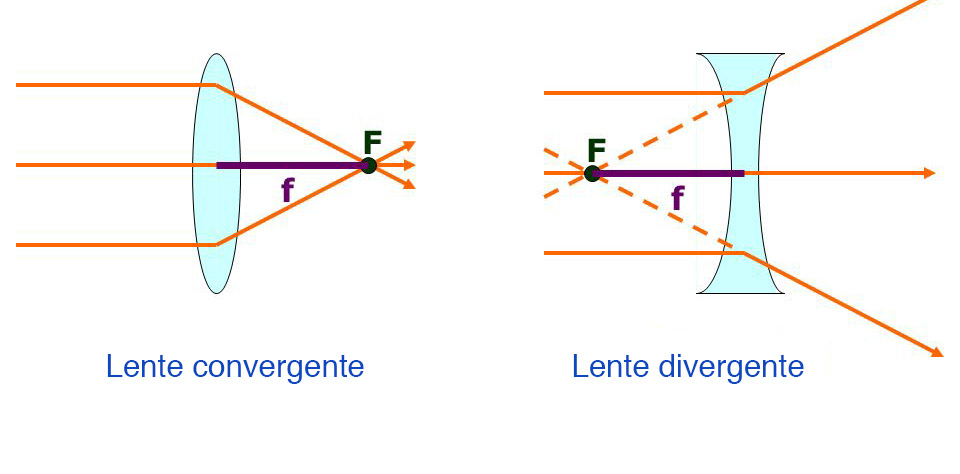
\includegraphics[scale=0.30]{tipos_de_lentes}
\begin{gather*}
  \frac{y\prime}{y} = \frac{s\prime}{s} \\
  \frac{1}{s\prime} - \frac{1}{s} = \frac{1}{f\prime}=P\\
\end{gather*}


\vspace{-15px}
\section{Física cuántica}
\subsection{Efecto fotoeléctrico}
\[E_{incidente} = E_{umbral}(W_{ext})+E_c\]
\[h\vartheta=h\vartheta_0+E_{cMax}\]
\[E_{cMax}=qV\]

\subsection{Dualidad onda/corpúsculo}

\[
  \begin{rcases}
    E=h\vartheta &\\
    E=mc^2 &\\
    c=\lambda\vartheta
  \end{rcases} h\frac{c}{\lambda}=mc^2;\ \frac{h}{\lambda}=mc; \ \frac{h}{\lambda}=p
\]

\subsection{Principio de indeterminación de Heisenberg}
\[
  \begin{cases}
    \Delta x\cdot\Delta p\geq\frac{h}{4\pi} &\\
    \Delta E\cdot\Delta t\geq\frac{h}{4\pi}  
  \end{cases}
\]

\section{Física nuclear}
\[M_{nuc}<Z\cdot m_p + (A-Z)\cdot m_n\]
\[\Delta m=M_{nuc} - [Z\cdot m_p + (A-Z)\cdot m_n]\]
\[E_{enlace}=\Delta mc^2\]
\[Estabilidad\rightarrow \frac{E_{enlace}}{A(nucleones)}\]

\subsection{Desintegración}
\[\lambda = \text{constante de desintegración}\]

Actividad: 
\[A=-\frac{dN}{dt}=\lambda N\]

Masa/núcleos en t: 
\[N=N_0 e^{-\lambda t}\]

Periodo de semidesintegración:
\[T_{\frac{1}{2}}\left(N=\frac{N_0}{2}\right)=\frac{\ln 2}{\lambda}\]

\[\text{Vida media:}\ \tau = \frac{1}{\lambda}\]
\[
\text{Leyes de desplazamiento:}
\begin{cases}
  \alpha\Rightarrow\prescript{A}{Z}{X}\rightarrow\prescript{4}{2}{\alpha}+\prescript{A-4}{Z-2}{Y}&\\
  \beta\Rightarrow\prescript{A}{Z}{X}\rightarrow\prescript{0}{-1}{\beta}+\prescript{A}{Z+1}{Y} &\\
  \gamma\Rightarrow\prescript{A}{Z}{X}^*\rightarrow\gamma+\prescript{A}{Z}{X}
\end{cases}
\]
\end{multicols}

\end{document}